\documentclass[11pt]{article}
\usepackage[a4paper,margin=1in]{geometry}
\usepackage{amsmath,amssymb}
\usepackage{graphicx}
\usepackage{hyperref}
\usepackage[strings]{underscore}

\title{Objective Clock Bases from Redundant Records\\Experiment Journal}
\author{Davut Emre Ta\c{s}ar}
\date{Started 20 June 2026}

\begin{document}
\maketitle

\section{Scope Freeze}

This project treats redundant records as a selector of an objective clock basis
under a fixed physical partition. The novelty target is not basis uniqueness
alone. The core distinction is between basis selection, label identification,
temporal order and temporal orientation.

The semantic freeze in ADR-000 is active. In particular, persistent trajectories
are chains in the record-dominance poset. Linear extensions of a branching poset
are scheduler totalizations and are not generally physical time trajectories.

\section{G0 Repository Readiness}

The repository was initialized on branch \texttt{implementation/g0-g1}. The
environment uses Python 3.13.11 with the project installed in editable mode.
Although the implementation contract targets Python 3.11/3.12, the package
declares \texttt{requires-python >=3.11}; the current environment is therefore a
valid but stricter compatibility check.

G0 outputs:
\begin{itemize}
  \item \texttt{results/processed/G0_environment_manifest.json}
  \item \texttt{results/processed/G0_file_manifest.json}
  \item \texttt{requirements.lock}
\end{itemize}

\section{G1 Theory and Exact Primitives}

\subsection{O1 Chain Characterization}

The generated T101 artifact checks 272 small distinct record codes and 188,158
candidate sequences. No mismatch was found between persistent sequences and
directed chains.

The diamond code has two maximal persistent chains and two linear extensions.
Both linear extensions force a record-loss edge between incomparable middle
snapshots, so the full persistent scalar-order count is zero.

\subsection{O1.1 Scalar Timeline Criterion}

The implementation emits a scalar timeline only when the quotient poset is total
and the original signatures are nonduplicate. Thermometer codes pass. Diamond,
duplicate and disconnected fixtures fail for the expected reasons.

\subsection{O2/O3 Capacity}

The binary capacity artifact confirms the exact bound
\[
N \le E + 1,
\]
with thermometer codes attaining equality. Boundary cases with
\(E=N-2\) fail as expected.

\begin{figure}[h]
\centering
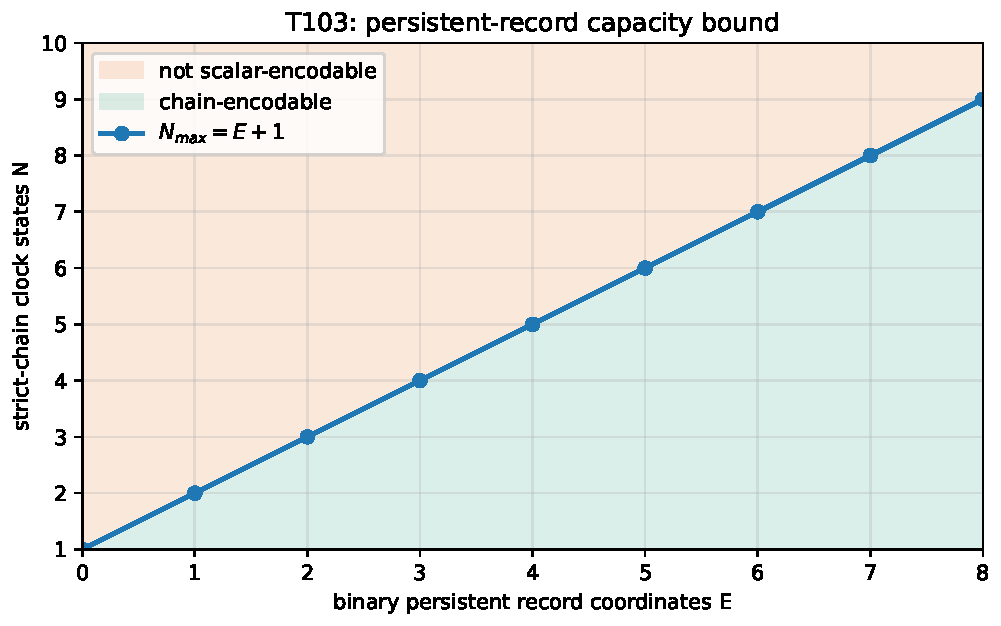
\includegraphics[width=0.72\linewidth]{../figures/fig_03_capacity.pdf}
\caption{Maximum strict-chain clock states for binary persistent records.}
\end{figure}

\subsection{O4 Noise Bound}

The generated grid compares exact majority decoding error with the Hoeffding
upper bound for odd \(q\) and \(p<1/2\). No bound violation was observed in the
G1 grid.

\subsection{No-Go Package}

The counterexample catalog records smallest explicit examples for label
permutation, orientation swap, unrestricted partition, single-fragment Bell
ambiguity and diamond branching without scalar time.

\section{Verification Log}

Latest G0/G1 verification:
\begin{verbatim}
ruff check .
pytest -q
mypy src/objective_clocks
\end{verbatim}

Result: 30 tests passed; ruff passed; mypy passed.

\section{Open Scientific Ambiguities Before G2}

No ambiguity blocks G2 at the current semantic layer. The main operational risk
for later stages is ensuring that classical experiment outputs continue to keep
maximal chains, linear extensions and automorphisms as separate quantities.

\section{G2 Batch 1: Classical Backbone}

\subsection{C0 Theorem Verification}

C0 was run from \texttt{configs/classical.yaml}. The output contains 42 grid
cells and 188,692 rows, with exhaustive binary maps in the configured small
state-space regime and frozen-seed random maps in larger cells. The theorem
failure count is zero. The output keeps maximal-chain count, linear-extension
count and automorphism count as separate columns.

\subsection{C1 Basis-Objectivity Landscape}

The Bell one-record control remains basis-ambiguous: the minimum and maximum
qubit-grid objectivity score are both 1.0. GHZ two-record objectivity selects the
Z basis with score 1.0, while the X-basis local objectivity score is 0.0. The
landscape is stored as NetCDF and rendered in
\texttt{figures/fig_02_basis_landscape.pdf}.

\subsection{C2 Order Reconstruction}

The order catalog includes thermometer, diamond, duplicate, disconnected,
orientation-free and erasure fixtures. The diamond fixture remains a branching
partial order, not a scalar timeline; no linear extension is marked as a physical
trajectory. Hasse diagrams are exported as GraphML.

\subsection{C3 Noise and Redundancy Sweep}

C3 ran the configured grid for \(N\in\{4,8\}\), seven odd redundancy values,
eight bit-flip probabilities and 10,000 trials per cell. All 112 grid cells are
complete. The exact binomial majority error never exceeds the Hoeffding upper
bound in the grid. The phase diagram is stored in
\texttt{figures/fig_04_noise_phase.pdf}.

\subsection{C4 Assumption Stress Tests}

C4 records five controls: Bell single-fragment ambiguity, GHZ two-fragment
positive control, dependent-fragment failure, degenerate-record failure and
unrestricted-partition failure. Each failed assumption maps to the predicted
failed conclusion.

\subsection{C5 Exact GHZ and Dephased Control}

C5 confirms that Z objectivity is identical for coherent GHZ and dephased
control states, while the global \(XXXX\) coherence witness distinguishes them.
The coherent GHZ value is numerically one and the dephased control value is zero.

\section{G3 Local Quantum Readiness}

\subsection{Q301 Circuit Family}

The four science circuits are frozen as untranspiled QPY payloads:
\texttt{ghz\_plus\_z}, \texttt{ghz\_plus\_x}, \texttt{ghz\_minus\_z} and
\texttt{ghz\_minus\_x}. The readout-calibration family contains eight
independent circuits. The circuit family contains no tomography. Qiskit
endianness is fixed by parsing bitstrings into logical order
\([C,S,R1,R2]\).

\subsection{Q302 Generic Noise Sweep}

The generic Aer sweep completes 100 grid cells over the configured one-qubit,
two-qubit and readout-error grid. Ninety-six cells pass the configured local
readiness thresholds. The results are stored in
\texttt{results/processed/Q1\_noise\_sweep.parquet}.

\subsection{Q303--Q304 Backend Selection and Local Twin}

The IBM Runtime credential is stored outside the repository in the local Qiskit
account file. The saved account is bound to the \texttt{open-instance} Open
Plan instance. Q303 performs provider listing and backend-property reads only;
it submits no workload. After the pre-result backend amendment, the current
provider snapshot selects
\texttt{ibm\_kingston}. The physical layout is \([125,117,126,124]\). The
native entangling gate is \texttt{cz}. The calibration timestamp is
\texttt{2026-06-20T22:25:00+03:00}.

Q304 builds a selected-layout aggregate depolarizing/readout proxy from that
snapshot and runs the planned local Aer workload. The local twin passes the
preregistered readiness thresholds with status
\texttt{backend\_snapshot\_ready}. This is not a hardware observation and does
not add Q-grade evidence.

\subsection{G3 Verification}

The G3 pipeline was rerun after documentation and manifest updates. Verification
passed with 43 tests, \texttt{ruff check .} clean and
\texttt{mypy src/objective\_clocks} clean. No provider job was submitted.

\section{A601 Claim Evidence Grading}

A601 generates \texttt{results/claim\_evidence\_matrix.csv}. The matrix assigns
evidence grades P, E, S, Q, I and N to every planned claim and records an
artifact-backed check plus a caveat for each row. The current matrix contains ten
claims: B0, O1, O2, O3, O4, N1, N2, N3, Q1 and Q2.

Unsupported claim count is zero. After H501/H502/H503, Q1 and Q2 receive
Q-grade evidence from the completed IBM four-qubit illustration. The Q-grade
rows are explicitly bounded: they do not promote the GHZ illustration into an
independent proof of the theorem-level claims. The classical/symbolic
contribution remains evaluated by proofs, exact checks and classical
experiments.

After A601 was added to the reproduction chain, \texttt{scripts/reproduce\_all.py}
completed successfully: pytest, G1, G2, G3, the G4 readiness audit, A601 and
the exact GHZ CLI all reran without failure.

\section{G4 Preregistration Freeze}

The G4 readiness audit now reaches \texttt{ready\_for\_h501}. H401 generated a
deterministic environment archive without recording secret values. H402 froze the
ISA circuit packet for the selected \texttt{ibm\_kingston} backend: 24 circuit
instances, 24,576 total shots, selected transpiler seed 0 and one QPY payload.

The H401 preregistration packet is frozen after explicit human approval. This
approval is only a preregistration freeze approval; it does not itself permit QPU
execution. The H403 dry-run confirms that the Open Plan instance is
\texttt{open-instance}, the ISA packet is present, human approval is recorded and
\texttt{ALLOW\_QPU\_EXECUTION} is not enabled. No Sampler was invoked and no
hardware job was submitted during G4.

\section{G5 Locked Hardware Path Before Execution}

Before any IBM execution, the repository now contains the complete H501--H503
code path. H501 submits exactly the frozen QPY workload through SamplerV2 only
when the frozen preregistration manifest, circuit-manifest hash, QPY hash, Open
instance metadata, clean repository state, preregistration tag and explicit
\texttt{ALLOW\_QPU\_EXECUTION=YES} gate all pass. It also refuses to run if a
previous H501 raw provider payload exists.

H502 computes the primary raw result from the downloaded provider bitstrings.
The raw decision uses the preregistered Clopper--Pearson and stratified
bootstrap rules, including the objectivity contrast, minimum Z correlation,
coherence contrast, GHZ-minus X-parity sign and no-single-block-dominance check.
H503 applies only the secondary independent tensor-product readout assignment
correction. The corrected result is reported beside the raw result and cannot
replace it.

\section{H501A1 Pre-Result Backend Amendment}

The first H501 job was accepted on \texttt{ibm\_marrakesh} but remained queued.
It was cancelled before any running timestamp, raw result download or QPU usage;
the provider metrics report zero quantum seconds. This cancellation therefore
does not constitute a hardware observation.

The backend change is treated as a protocol amendment. Q305 compared
\texttt{ibm\_kingston}, \texttt{ibm\_fez} and \texttt{ibm\_marrakesh} using
read-only provider metadata plus the same backend-derived local twin simulation.
All candidates passed the local twin gate. The replacement backend is
\texttt{ibm\_kingston}; Q303/Q304, H402 ISA generation, H401 preregistration
freeze, H403 dry-run and H404 tagging are regenerated for the replacement before
any amended H501 execution.

\section{G5 Hardware Execution and Locked Analysis}

The amended H501 job completed on \texttt{ibm\_kingston} with job id
\texttt{d8rfasuab0ds73drkaig}. The job used the H501A1-regenerated
preregistration packet.
\begin{itemize}
  \item Preregistration tag: \texttt{v0.4-qpu-preregistered-kingston}
  \item Circuit instances: 24
  \item Observed shots: 24,576
\end{itemize}
\begin{itemize}
  \item Created: \texttt{2026-06-20T20:17:55.809388Z}
  \item Running: \texttt{2026-06-20T20:17:57.209474Z}
  \item Finished: \texttt{2026-06-20T20:18:10.354081Z}
  \item Quantum usage: 9 seconds
\end{itemize}
The raw payload is stored in
\path{results/raw/H501_provider_payload_d8rfasuab0ds73drkaig.json}.

H502 is the primary result. It reads the downloaded provider bitstrings and
applies the preregistered raw inclusion rule without mitigation. The raw result
passes main-text inclusion:
\texttt{passes\_main\_text\_inclusion\_without\_mitigation=true}. The
bootstrap lower confidence bounds use seed \texttt{20260621} and 10,000
replicates. The objectivity contrast lower bound is
\(0.8876953125\), the minimum Z-correlation lower bound is
\(0.9169542107266444\) and the coherence contrast lower bound is
\(0.877685546875\). The GHZ-plus, GHZ-minus and mixture X-parity witnesses are
\(0.8955078125\), \(-0.87744140625\) and \(0.009033203125\). No single
randomized block dominates the objectivity or coherence contrast.

H503 is secondary robustness evidence only. The independent tensor-product
readout assignment correction has condition number \(1.1172921620957568\),
passes the corrected point thresholds and agrees qualitatively with the raw
result. The corrected point estimates are \(\Delta_{\mathrm{obj}} =
0.9850328718815358\) and \(\Delta_{\mathrm{coh}} =
0.9687926905262139\). H503 cannot replace the raw H502 decision; the primary
inclusion result remains raw.

\end{document}
